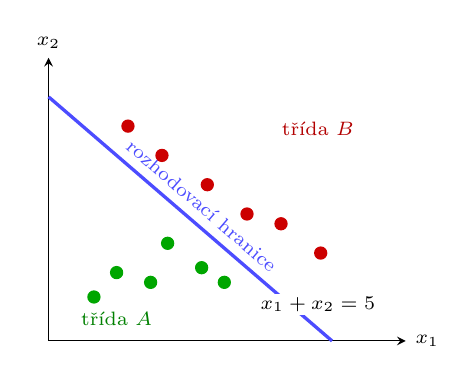
\begin{tikzpicture}[x=0.72cm,y=0.62cm,>=stealth]

    % Osy
    \draw[->] (0,0) -- (6.3,0)
        node[right, font=\scriptsize] {$x_1$};

    \draw[->] (0,0) -- (0,5.8)
        node[above, font=\scriptsize] {$x_2$};

    % Rozhodovací hranice x_1 + x_2 = 5
    \draw[very thick, blue!70]
    (0,5)
    --
    node[
        midway,
        sloped,
        above,
        font=\scriptsize,
        text=blue!70
    ] {rozhodovací hranice}
    (5,0);

    % Třída A
    \foreach \x/\y in {
        0.8/0.9,
        1.2/1.4,
        1.8/1.2,
        2.1/2.0,
        2.7/1.5,
        3.1/1.2
    }{
        \fill[green!65!black] (\x,\y) circle (2.4pt);
    }

    % Třída B
    \foreach \x/\y in {
        1.4/4.4,
        2.0/3.8,
        2.8/3.2,
        3.5/2.6,
        4.1/2.4,
        4.8/1.8
    }{
        \fill[red!80!black] (\x,\y) circle (2.4pt);
    }

    % Popisky oblastí
    \node[font=\scriptsize, green!50!black]
        at (1.2,0.45) {třída $A$};

    \node[font=\scriptsize, red!70!black]
        at (4.75,4.35) {třída $B$};

    % Rovnice hranice
    \node[
        font=\scriptsize,
        fill=white,
        inner sep=1pt
    ] at (4.75,0.75)
        {$x_1+x_2=5$};

\end{tikzpicture}
